% ============================================================================ COMPARE
\section{Comparing Integrations}\label{sec:compare}

In comparison mode the same synthesized regulator---cell count, topology, devices, passives and
tier stack---is placed in each integration, and every output is reported inside declared loss
boundaries. Because the integrations differ in how the converter can be cooled, they are compared
three ways (Table~\ref{tab:compare}, Fig.~\ref{fig:tiers}): at one common temperature, which is
what an analysis without electrothermal coupling sees; with the same top cold plate (cooling~A);
and with the same top plate and an identical bottom plate under the cell grid, behind the same
50-\textmu m thermal interface as the top plate (cooling~B). Model-form errors common to all
columns---the converter loss model, the device temperature coefficients, the solder
law---largely cancel in the differences.

% GENERATED by scripts/tcpmt_manuscript_macros.py -- do not edit
\begin{table*}[!t]
\caption{The three integrations at S0 under cooling~A (one top cold plate) and cooling~B (top and bottom plates), reference capacitor case A0. Loss inside the package-internal boundary unless stated; $\pm U$: numerical uncertainty (Table~\ref{tab:uncertainty}).}
\label{tab:compare}
\centering
\footnotesize
\setlength{\tabcolsep}{3.5pt}
\begin{tabular}{@{}lrrrrrr@{}}
\toprule
 & \multicolumn{3}{c}{Cooling A: top plate} & \multicolumn{3}{c}{Cooling B: top and bottom plates}\\
\cmidrule(lr){2-4}\cmidrule(l){5-7}
 & Z1 & Z2 & Z3 & Z1 & Z2 & Z3 \\
\midrule
\multicolumn{7}{@{}l}{\emph{Performance}}\\
Loss (W) & 144.3$\pm$1.7 & 147.4$\pm$1.5 & 199.6$\pm$2.0 & 142.6$\pm$1.6 & 115.2$\pm$1.2 & 124.5$\pm$1.2 \\
\quad conversion / routing & 140.7 / 3.6 & 144.8 / 2.7 & 181.4 / 18.1 & 139.1 / 3.6 & 112.9 / 2.3 & 109.7 / 14.8 \\
Peak temperature ($^\circ$C) & 115.7 & 124.3 & 185.8 & 111.3 & 81.5 & 83.3 \\
GaN junction, bound ($^\circ$C) & 116.2 & 124.8 & 186.3 & 112.3 & 67.6 & 61.0 \\
Board, mean ($^\circ$C) & 111 & 93 & 131 & 67 & 75 & 72 \\
Die warpage (\textmu m) & 25.5$\pm$1.5 & 68.7$\pm$1.1 & 59.5$\pm$9.5 & 5.9$\pm$0.3 & 17.6$\pm$0.3 & 7.1$\pm$1.1 \\
$\du$ (\textmu m) at $T_{\mathrm{j}}$ ($^\circ$C) & 2.21 (115.0) & 3.09 (97.2) & 4.47 (109.9) & 0.69 (108.3) & 2.10 (78.7) & 1.56 (80.4) \\
$\deps$ ($10^{-3}$/cycle)\textsuperscript{a} & 5.73$\pm$0.17 & 8.02$\pm$0.08 & 13.48$\pm$0.27 & 1.89$\pm$0.14 & 4.04$\pm$0.13 & 2.32$\pm$0.12 \\
Heat to top / bottom plate (W) & 1144 / 0 & 1147 / 0 & 1198 / 0 & 1130 / 13 & 925 / 190 & 960 / 164 \\
\midrule
\multicolumn{7}{@{}l}{\emph{Loss accounting and platform}}\\
Static 1-V drop to the die (mV)\textsuperscript{b} & 0.04 & 0.83 & 16.0 & 0.04 & 0.78 & 13.3 \\
Feed limit $R^*$ (m$\Omega$) & n/a & none & none & n/a & 48.4 & 32.1 \\
Physical feed loss (W) & -- & 1.17 & 0.12 & -- & 1.10 & 0.10 \\
Pumping, shaft (W) & 31 & 31 & 31 & 61 & 61 & 61 \\
Platform-inclusive loss (W) & 174.9 & 179.2 & 230.2 & 203.8 & 177.4 & 185.7 \\
\midrule
\multicolumn{7}{@{}l}{\emph{Feasibility}}\\
All component and material limits & pass & pass & \textbf{fail} & pass & pass & pass \\
Joint within solder law ($\le125\,^\circ$C) & pass & pass & pass & pass & pass & pass \\
BGA sites carrying power (of 1369) & 108 & 0 & 1334\textsuperscript{c} & 108 & 0 & 1334\textsuperscript{c} \\
Worst via aspect ratio, A0 / A1 & 0.83 / 8.6 & 0.83 / 8.6 & 0.83 / 8.6 & 0.83 / 8.6 & 0.83 / 8.6 & 0.83 / 8.6 \\
Fits the 2.4-mm board opening, A1 & n/a & \textbf{no} & n/a & n/a & \textbf{no} & n/a \\
\bottomrule
\end{tabular}
\par\smallskip\raggedright\footnotesize \textsuperscript{a}Stabilized cycle, L0 mesh. \textsuperscript{b}1-V conductor loss divided by the load current. \textsuperscript{c}Leaves 35 sites for every signal and auxiliary rail: a feasibility failure of this package.  A1: rated MLCC flying capacitors (1030-\textmu m tier).
\end{table*}


\subsection{Placement alone}\label{sec:compare-elec}
At a common temperature the conversion loss is identical by construction, and the integrations
differ only in routing (Fig.~\ref{fig:loss}). Moving the regulator out of the package removes
the package 48-V network, \PhvZone~W in Z1, and sends the kiloampere 1-V current through new
conductors: the Cu-pillar attach and the TSV field in Z2 (\PattZtwo{} and \PtsvZtwo~W), and the
board-level attach, the board via field with the ball field, and the TSVs in Z3 (\PattZthree,
\PboardZthree{} and \PtsvZthree~W). At 100\,$^\circ$C, Z2 is \GapIsoHotZtwo~W below Z1 and Z3
\GapIsoHotZthree~W above it. Z3 pays more than its ledger shows. At 1.5~A per ball its 1-V
current needs 1334 of the 1369 sites of the 0.8-mm ball array, leaving 35 for every signal and
auxiliary rail, and only \LandBallsInside{} balls per rail lie under the cells. The current of
the rest must spread laterally in the land side of the package; a sheet solution of that
redistribution, which the coupled ledger does not contain, adds \LandPmin--\LandPmax~W and
\LandDVmin--\LandDVmax~mV of drop for \LandTmax--\LandTmin~\textmu m of land-side copper.
Carrying the current straight down under the cells would require a ball pitch of
\PitchMaxZthree~mm.

\begin{figure}[!t]
\centering
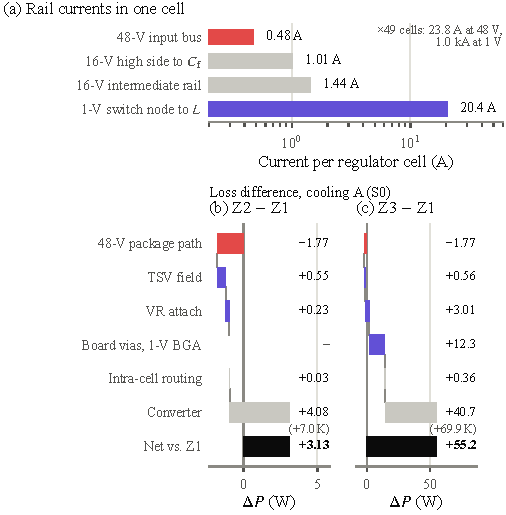
\includegraphics[width=\columnwidth]{fig5_loss_swap.pdf}
\caption{(a) Current per regulator cell in each class of connection, by rail. (b), (c)
Package-internal loss of Z2 and of Z3 minus that of Z1 under cooling~A, term by term: the routing
each integration removes or adds, and the change of conversion loss caused by the converter's own
temperature (low-side tier temperature difference in parentheses).}
\label{fig:loss}
\end{figure}

\subsection{The same top cold plate}
With one top plate the converter's thermal path decides the ranking, and it reverses the
placement-alone result twice. The converter of Z2 is cooled only through the attach and the
substrate, so its low-side tier runs \dTlsAbsZtwoSzero~K hotter than in Z1 and its conversion loss
rises by \dPconvAbsZtwoSzero~W, about \ConvToRouteZtwo{} times the \dProuteAbsZtwoSzero~W it saves
in routing: Z1 has the lower loss, by \GapAZtwo~W. The converter of Z3 must push its heat up
through 2.4~mm of board: it reaches \TmaxAZthree\,$^\circ$C and dissipates \PlossAZthree~W,
\GapAZthree~W more than Z1. The cooling solution of the embedded and package-backside
integrations does not survive the board-backside one. Mechanically, Z1 sandwiches the converter
between the die and the substrate on the full ball array and its die warps by \WarpAZone~\textmu m;
Z2 is a thin silicon plate that carries the encapsulated converter on one side and rests on a
ring of balls around the opening, a bimetal strip whose die warps \WarpRatioZtwo{} times as much
and whose critical joint moves \DuRatioZtwo{} times as far (Fig.~\ref{fig:fields}).
% TODO(data): Z3 under cooling A, mechanical sentence

\begin{figure*}[!t]
\centering
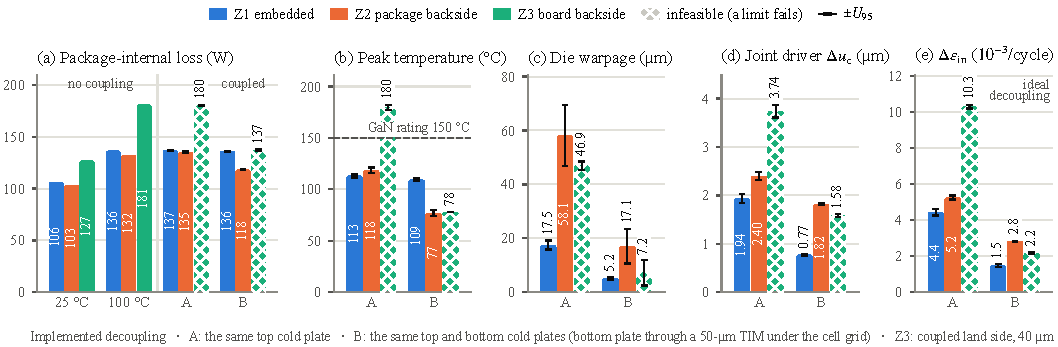
\includegraphics[width=\textwidth]{fig8_tiers.pdf}
\caption{The three integrations at S0 compared three ways. (a) Package-internal loss at one
common temperature (no electrothermal coupling) and coupled under cooling~A (the same top cold
plate) and cooling~B (the same top and bottom plates). (b) Peak temperature, (c) die warpage and
(d) critical-joint displacement under cooling~A and~B. Open diamonds: the interface-free bottom
plate, a bound.}
\label{fig:tiers}
\end{figure*}

\subsection{The same top and bottom cold plates}
% TODO(data): cooling B results -- which integration can use the bottom plate (Z1 only through
% substrate, balls and 2.4 mm of board; Z2 and Z3 directly), losses, temperatures, warpage, joints;
% the interface-free bound; R* under B.

The direct 48-V feed of the backside integrations lies outside the package boundary; its loop
resistance enters through~\eqref{eq:feed} and is treated as a requirement (Fig.~\ref{fig:feed}).
Where a backside regulator is ahead at zero feed resistance, $R^*$ is the largest loop resistance
that keeps it ahead; where it is behind, no feed recovers the difference. Under cooling~A, Z2 is
behind at S0 and needs a loop below \RstarZtwoSone~m$\Omega$ at S1, about \RstarOverLoopZtwo{}
times the package 48-V loop of Z1 (\RloopZone~m$\Omega$).

\begin{figure}[!t]
\centering
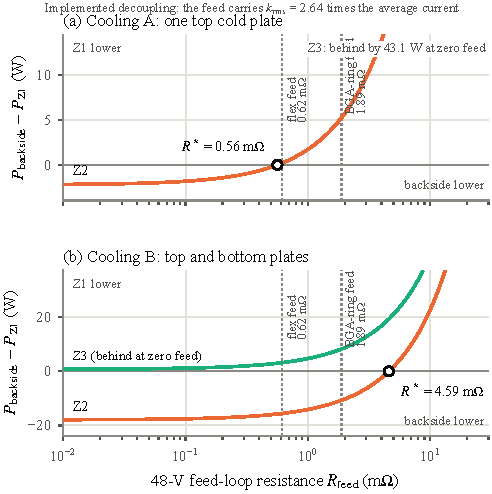
\includegraphics[width=\columnwidth]{fig6_crossover.pdf}
\caption{Platform-inclusive loss of the directly fed backside integrations minus that of Z1,
against the external feed-loop resistance. (a) S0. (b) S1. Below zero the backside integration
has the lower platform-inclusive loss; circles mark the crossover $R^*$. Dashed: the package
48-V loop resistance of Z1, for scale.}
\label{fig:feed}
\end{figure}
